\documentclass[12pt,a4paper]{article}
%\usepackage[utf8]{inputenc}
%\usepackage[portuguese]{babel}
\usepackage{amsmath, amsfonts, amssymb}
\usepackage{graphicx}
\usepackage[utf8]{inputenc} % Permite utilizar caracteres especiais: Ex: ç á à...
\usepackage[onehalfspacing]{setspace} % Espaçamento de 1,5
\usepackage[caption=false]{subfig}
\usepackage{cabecalho}
\usepackage{multirow}
\usepackage{float}
\usepackage[lmargin=3cm, tmargin=3cm, rmargin=2cm, bmargin=2cm]{geometry}
\usepackage{indentfirst}
\usepackage{IEEEtrantools}


\newcommand{\trans}{\mathsf{T}}
\newcommand{\hermit}{\mathsf{H}}
\newcommand{\mc}[1]{\ensuremath{\mathcal{#1}}}
\newcommand{\mbb}[1]{\ensuremath{\mathbb{#1}}}
\newcommand{\Natural}{\mathbb{N}}
\newcommand{\Integer}{\mathbb{Z}}
\newcommand{\Irrational}{\mathbb{I}}
\newcommand{\Rational}{\mathbb{Q}}
\newcommand{\Real}{\mathbb{R}}
\newcommand{\Complex}{\mathbb{C}}
\newcommand{\obs}[1]{\textcolor{red}{(#1)}}
\newcommand{\sizecorr}[1]{\makebox[0cm]{\phantom{$\displaystyle #1$}}} % Used to seize the height of equation

\begin{document}
\initcab{Universidade Federal do Ceará}{Filtros Adaptativos}{Charles Casimirio}{519024}{\today}{Lista 04}

\section{Question 1}

For a adaptive filter where the input signal is given by \(x(n) = \cos(\frac{\pi n}{3})\) and the desired signal is \(d(n) = x(n+1)\), it is used the RLS algorithm with a forgetting factor of \(\lambda = 0.98\). The signal output, \(y(n)\), is shown in Figure \ref{fig:signal-prediction} in addition to the input signal, \(x(n)\).
\begin{figure}[H]
    \centering
    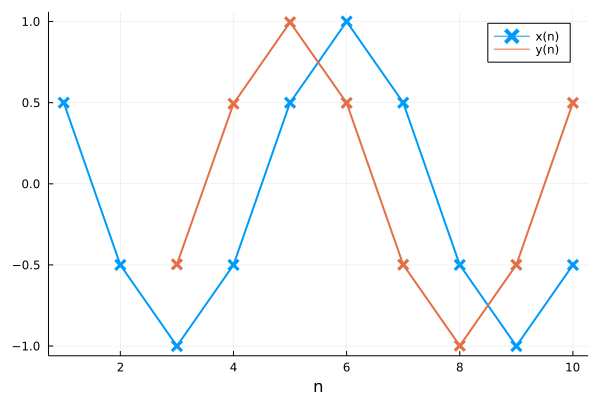
\includegraphics[scale=.4]{../figs/q1.png}
    \caption{Value of \(x(n)\) and its predicted value.}
    \label{fig:signal-prediction}
\end{figure}

\section{Question 2}

Let \(s(n)\) be a white Gaussian noise that passes through a channel whose transfer function is given by
\begin{align}
    H(z) = 1 + 1.6z^{-1}.
\end{align}
The signal output, \(x(n) = s(n) + 1.6s(n-1)\), passes through an equalizer that uses the RLS algorithm with a forgetting factor of \(0.99\) to retrieve the transmitted signal. The Figure \ref{fig:channel-predicted-coeff} shows the learning step of the coefficient vector, \(\mathbf{w}(n)\), throughout the iterations. The Wiener solution is also plotted as a reference.
\begin{figure}[H]
    \centering
    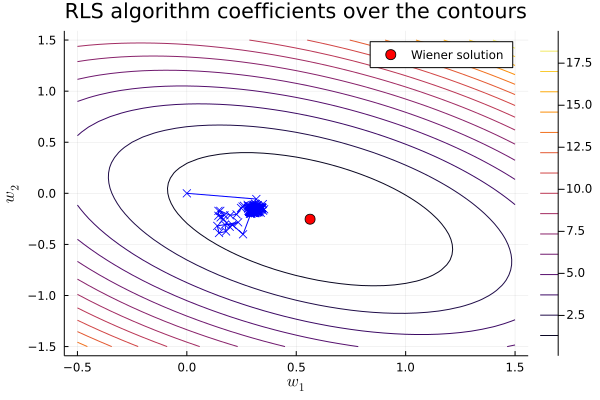
\includegraphics[scale=.4]{../figs/q2_contour.png}
    \caption{predicted coefficients.}
    \label{fig:channel-predicted-coeff}
\end{figure}

The filter output and the desired sinal is shown in the Figure \ref{fig:channel-output}, and the MSE (mean squared error) of this algorithm is shown in Figure \ref{fig:mse}
\begin{figure}[H]
    \centering
    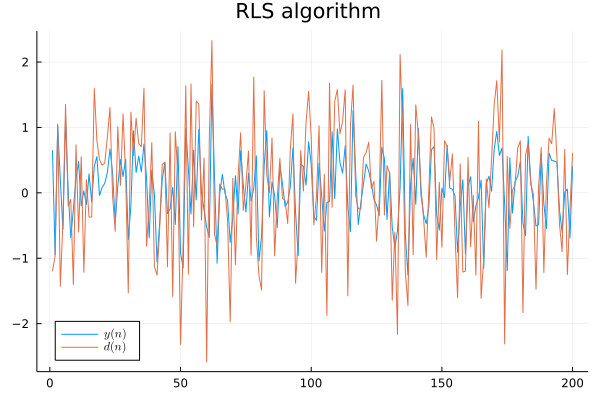
\includegraphics[scale=.4]{../figs/q2_rls_algorithm_output.png}
    \caption{Filter output.}
    \label{fig:channel-output}
\end{figure}

\begin{figure}[H]
    \centering
    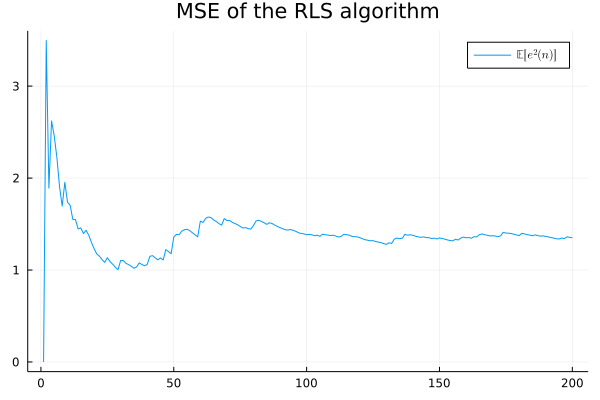
\includegraphics[scale=.4]{../figs/q2_rls_algorithm_error.png}
    \caption{Filter output.}
    \label{fig:mse}
\end{figure}


\section{Question 5}

The RLS algorithm with a forgetting factor of \(0.9\), \(0.99\), and \(0.999\) was computed for the same adaptive equalization problem of the homework 03. The model was trained with 500 symbols of a 4-QAM (Quadrature Amplitude Modulation) constellation. Then, the receiver operates in decision-directed mode for a 16-QAM scheme, under a SNR (Signal-to-Noise Ratio) of 30 dB. The result is obtained for \(\lambda \in \left\{ 0.9, 0.99, 0.999 \right\}\). The signal input, \(x(n)\), the transmitted symbol, \(s(n)\), and its estimate, \(\hat{s}(n)\) are shown in Figure \ref{fig:system-equalizer-output}.

It is possible to see that the receiver can retrieve the transmitted symbol for all values of \(\lambda\). Their convergences, however, vary with the value of \(\lambda\), as shown in Figure \ref{fig:equalizer-error}.

\begin{figure}[H]
    \centering
    \subfloat[\centering \(\lambda = 0.9\)]{%
      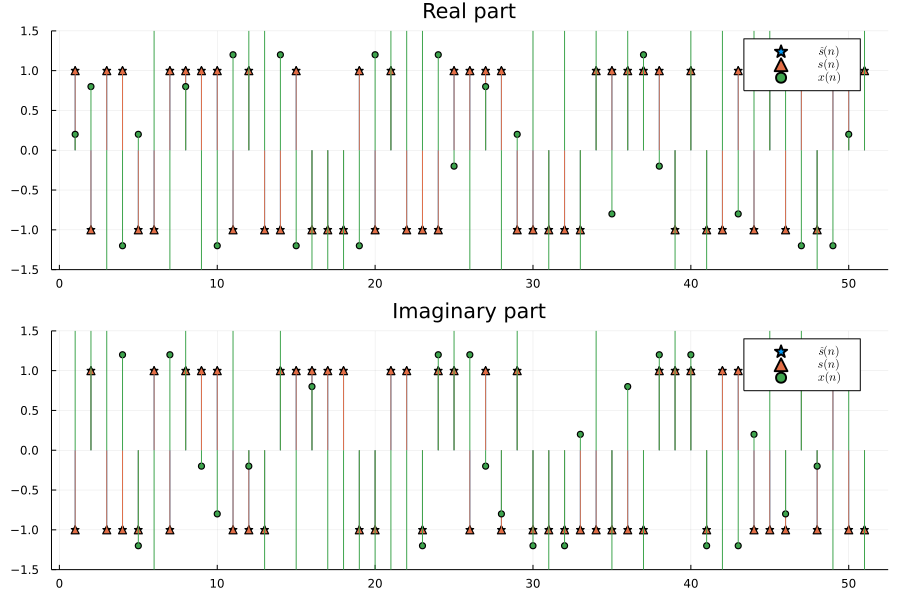
\includegraphics[clip,width=0.6\columnwidth]{../figs/q5_output_lambda0.9.png}%
      \label{fig:itema}
    }
    
    \subfloat[\centering \(\lambda = 0.99\)]{%
      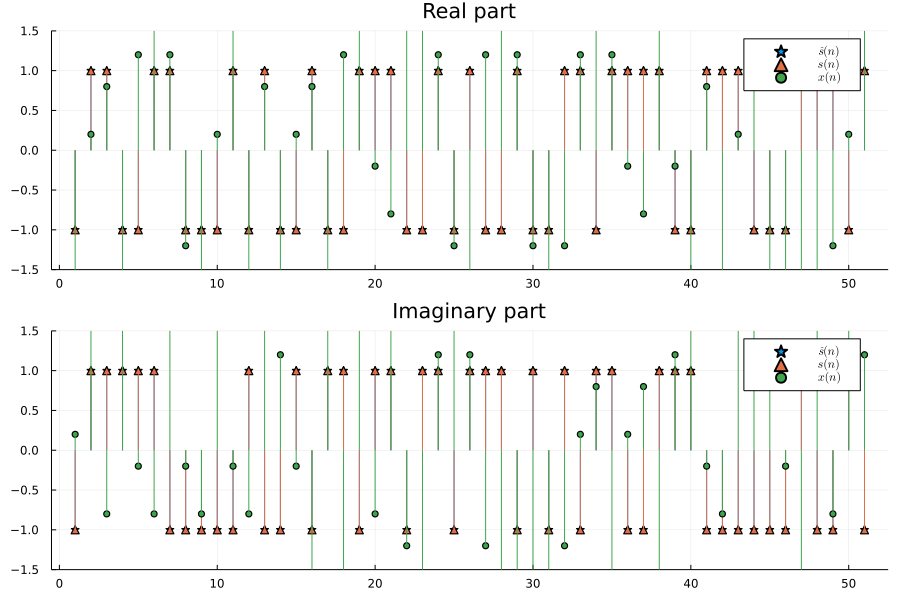
\includegraphics[clip,width=0.6\columnwidth]{../figs/q5_output_lambda0.99.png}%
      \label{fig:itemb}
    }
    
    \subfloat[\centering \(\lambda = 0.999\)]{%
      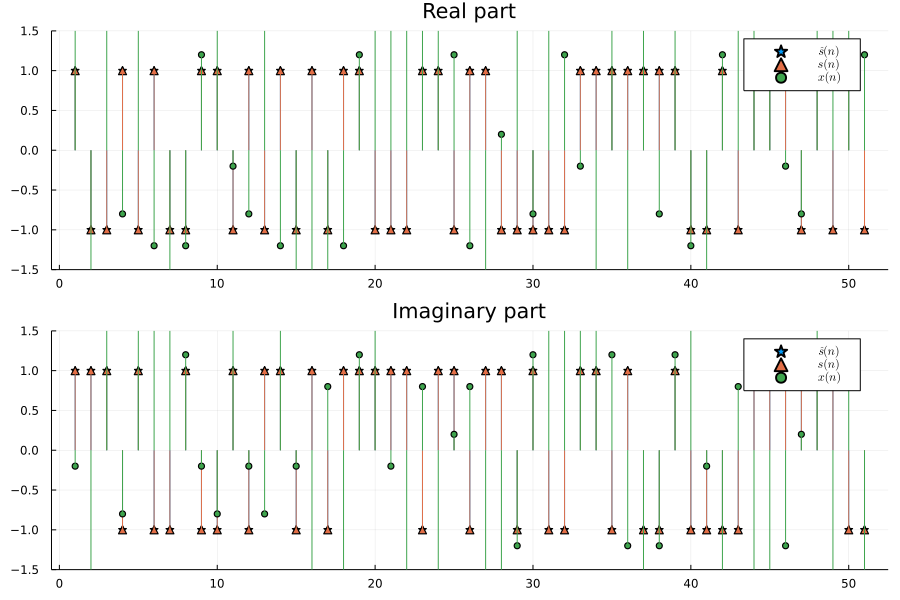
\includegraphics[clip,width=0.6\columnwidth]{../figs/q5_output_lambda0.999.png}%
      \label{fig:itemb}
    }
    
    \caption{main caption}
    \label{fig:system-equalizer-output}
\end{figure}

\begin{figure}[H]
    \centering
    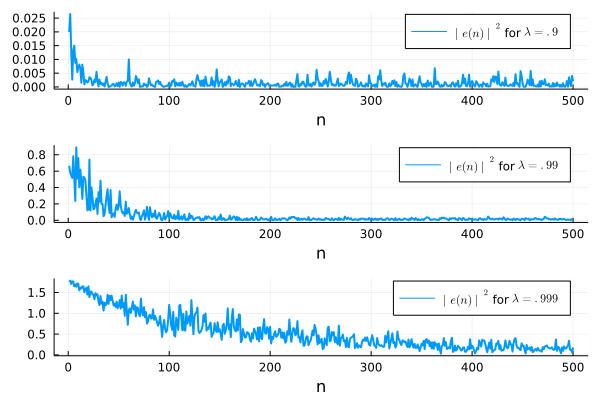
\includegraphics[scale=.6]{../figs/q5_error_signal.png}
    \caption{The absolute value of the error signal, \(e(n) = d(n) - y(n)\), for different values of \(\lambda\).}
    \label{fig:equalizer-error}
\end{figure}


% \bibliography{ref.bib}
% \bibliographystyle{ieeetr}

\end{document}